\section{MCMC}
\begin{frame}
  \frametitle{MCMC概述}
  \begin{itemize}
    \item MCMC由两个MC组成,即蒙特卡罗方法(Monte Carlo Simulation,MC)和马尔科夫链(Markov Chain,MC)。MCMC是很多算法求解的基础。
  \end{itemize}
\end{frame}

\begin{frame}
  \frametitle{蒙特卡罗方法}
  \begin{itemize}
    \item MCMC由两个MC组成,即蒙特卡罗方法(Monte Carlo Simulation,MC)和马尔科夫链(Markov Chain,MC)。MCMC是很多算法求解的基础。
  \end{itemize}
\end{frame}

\begin{frame}
  \frametitle{概率分布采样}
  \begin{itemize}
    \item 对于常见的均匀分布Uniform(0,1)是容易得到采样样本的,一般通过线性同余发生器就可以很方便的生成(0,1)之间的伪随机数样本。
    \item 而其他常见的概率分布,无论是离散的分布还是连续的分布,它们的样本都可以通过Uniform(0,1)的样本转换而得。
          比如二维正态分布的样本$(Y1, Y2)$可以通过独立采样得到。Uniform(0,1)样本对$(X1, X2)$通过如下的式子转换而得:
          \begin{equation}
            \begin{cases}
              Y1 = \sqrt{-2\ln{X1}} \cos{(2\pi X2)} \\
              Y2 = \sqrt{-2\ln{X2}} \sin{(2\pi X2)}
            \end{cases}
          \end{equation}
    \item 其他一些常见的连续分布,比如t分布,F分布,Beta分布,Gamma分布等,都可以通过类似的方式从Uniform(0,1)得到的采样样本转化得到。
    \item 很多时候我们的$x$的概率分布并不是常见的分布,这意味着我们没法方便的得到这些非常见的概率分布的样本集。那这个问题怎么解决?
  \end{itemize}
\end{frame}

\begin{frame}
  \frametitle{接受-拒接采样}
  \begin{itemize}
    \item 对于概率分布不是常见的分布,一个可行的办法是采用接受-拒绝采样来得到该分布的样本。
    \item 假设存在一个分布$p(x)$太复杂在程序中没法直接采样,那么设定一个程序可采样的分布 $q(x)$ 比如高斯分布,然后按照一定的方法拒绝某些样本,
          以达到接近 $p(x)$ 分布的目的,其中$q(x)$叫做建议分布(Proposal Distribution)。
    \item 具体采用过程:设定一个方便采样的常用概率分布函数 $q(x)$,以及一个常量 $k$,使得 $p(x)$ 总在 $kq(x)$ 的下方。如下图。

  \end{itemize}

\end{frame}

\begin{frame}
  \frametitle{接受-拒接采样}
  \centering
  \begin{figure}
    
    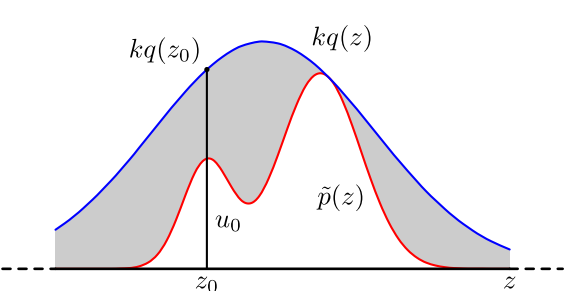
\includegraphics[width=8cm,trim=0 0 0 0,clip]{mcmc/jiesoujujue.png}
    \caption{拒接-接受采样示意图}
  \end{figure}
  
  % \begin{itemize}
  %   \item  首先,采样得到𝑞(𝑥)的一个样本𝑧0,方法用概率分布采样。然后,从均匀分布$(0, kq(z_0))$中采样得到一个值$𝑢$。
  %          如果$u$落在了上图中的灰色区域,则拒绝这次抽样,否则接受这个样本$z_0$。
  %          重复以上过程得到n个接受的样本$z_0, z_1, z_{n-1}$则最后的蒙特卡罗方法求解结果为:$$\frac{1}{n}\sum_{i=0}^{n-1} \frac{f(z_i)}{p(z_i)}$$
  %          整个过程中,我们通过一系列的接受拒绝方法来达到用$q(x)$模拟$p(x)$概率分布的目的。
  % \end{itemize}
\end{frame}

\begin{frame}
  \frametitle{接受-拒接采样}
  % 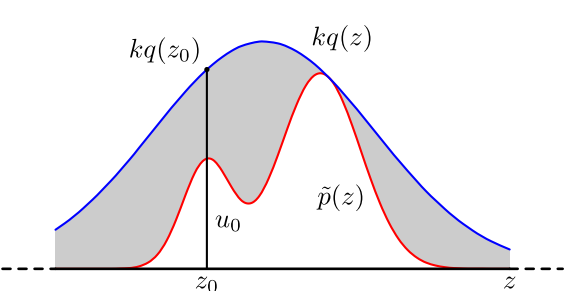
\includegraphics[width=5cm,trim=0 0 0 0,clip]{mcmc/jiesoujujue.png}
  \begin{itemize}
    \item  首先,采样得到𝑞(𝑥)的一个样本𝑧0,方法用概率分布采样。然后,从均匀分布$(0, kq(z_0))$中采样得到一个值$𝑢$。
           如果$u$落在了上图中的灰色区域,则拒绝这次抽样,否则接受这个样本$z_0$。
           重复以上过程得到n个接受的样本$z_0, z_1, ..., z_{n-1}$则最后的蒙特卡罗方法求解结果为:$$\frac{1}{n}\sum_{i=0}^{n-1} \frac{f(z_i)}{p(z_i)}$$
           整个过程中,我们通过一系列的接受拒绝方法来达到用$q(x)$模拟$p(x)$概率分布的目的。
  \end{itemize}
\end{frame}

\begin{frame}
  \frametitle{蒙特卡罗方法小结}
  \begin{itemize}
    \item 使用接受-拒绝采样,我们可以解决一些概率分布不是常见的分布的时候,得到其采样集并用蒙特卡罗方法求和的目的。
    但是接受-拒绝采样也只能部分满足我们的需求,在很多时候我们还是很难得到我们的概率分布的样本集。比如:
    \begin{enumerate}
      \item 对于一些二维分布$p(x, y)$,有时候我们只能得到条件分布$p(x|y)$和$p(y|x)$和,却很难得到二维分布$p(x,y)$一般形式,
      这时我们无法用接受-拒绝采样得到其样本集。
      \item 对于一些高维的复杂非常见分布$p(x_1, x_2, ..., x_n)$我们要找到一个合适的$q(x)$和$k$非常困难。
    \end{enumerate}
    \item 从上面可以看出,要想将蒙特卡罗方法作为一个通用的采样模拟求和的方法,必须解决如何方便得到各种复杂概率分布的对应的采样样本集的问题。
  \end{itemize}

\end{frame}